%----------------------------------------
% Write your notes here
%----------------------------------------

\section{Introduction/Recap}

Last week the class was introduced to causality and experiments by Andrew and Amit, Microsoft Researchers who were the guest lecturers.  Today, the lecture focuses more in-depth on these concepts. First we discussed random experiments, highlighting why they are great in theory, why they can be troublesome in practice, and what you can do to not fall prey to these problems.  Next we discussed different designs of natural experiments, as well as some caveats. Finally, we explored some recent work Professor Hofman has been undertaking with Amit regarding discovering natural experiments.

\section{Random Experiments}
\subsection{Review example from last lecture}

If we want to assess the effect of hospitalization on health, we must account for confounds: the cause and effect may be confounded by a common cause, and be changing together as a result.  Figure 1 displays this idea: our health today has an effect on our hospitalization today, as well as our health tomorrow. 

\begin{figure}[ht]
  \begin{center}
    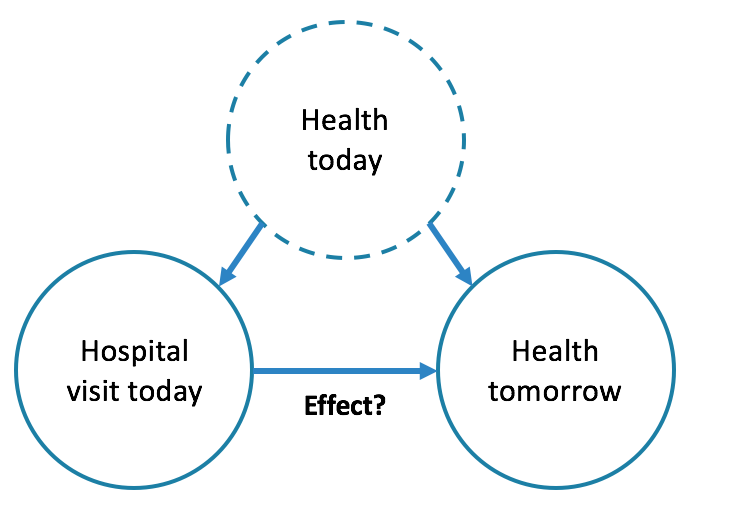
\includegraphics[width=0.3\textwidth]{figures/fig1}
        \caption{Effect and cause may be confounded by a common cause \textit{ Source: lecture 11 slides}}
    \label{figure 1}
  \end{center}
\end{figure}

As Box explains, "to find out what happens when you change something, it is necessary to change it." 

\subsection{Random assignment}
Through \textbf{random assignment} we are able to break this link between the confound and the second event (the thing we care about).  Through intervention, say a coin flip as in figure 2, we are able to determent treatment independent of any confounds.\\ 

\begin{figure}[ht]
  \begin{center}
    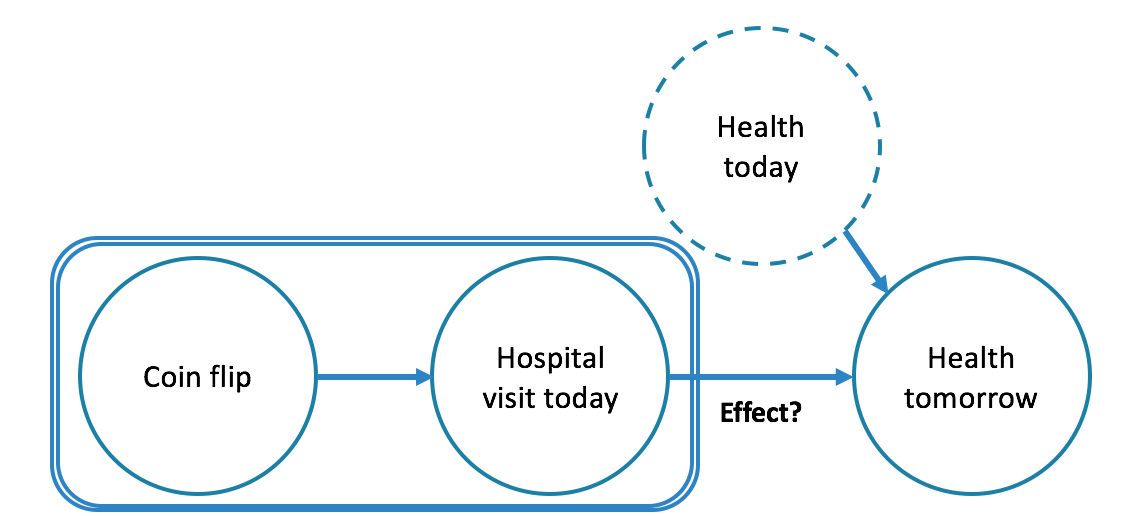
\includegraphics[width=0.3\textwidth]{figures/fig2}
        \caption{Through intervention, we can break the link between the confounded thing and what we care about \textit{ Source: lecture 11 slides}}
    \label{figure 2}
  \end{center}
\end{figure}

Under this approach, we are not able to see what didn't happen, a concept that is referred to as \textbf{counterfactuals}.  To isolate the causal effect, we have to change one and only one thing, and then compare the outcomes.  All else must be equal; while this is possible with experiments where we can ensure identical formats and procedures are followed, we cannot do this with people. \\

\textbf{Random Assignment} is the process of assigning one of two worlds to an instance and observing what happens.  The groups in each of these two worlds are only different in what treatment they receive.  Neyman's Model does a great job in understanding why randomization works, which will later help us in understanding instrumental variables in natural experiments.  In Figure 3, each person $i$ is represented by two tickets: $T_i$ representing what happens under treatment, and $C_i$ representing what happens under control.  When we draw a random sample, for those in the treatment group, we only observe the $T_i$ outcome, and vice versa for the control group.  Random assignment is usually presented as conditional expectations, but Neyman's model is a simpler and intuitive explanation. 

\begin{figure}[ht]
  \begin{center}
    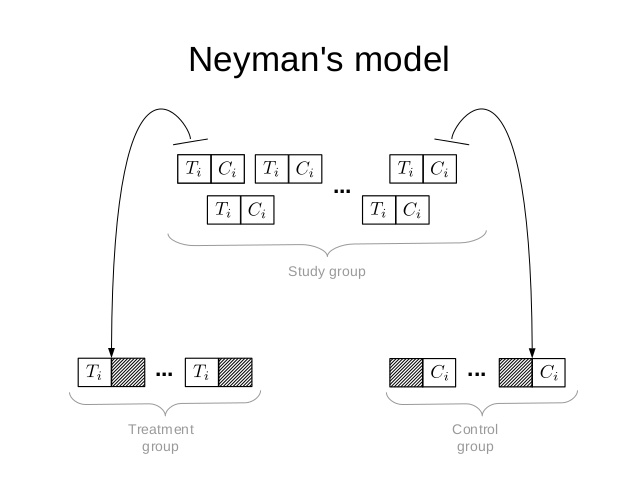
\includegraphics[width=0.5\textwidth]{figures/fig3}
        \caption{Neyman's Model  \textit{ Source: https://www.slideshare.net/ChaToX/natural-experiments}}
    \label{figure 3}
  \end{center}
\end{figure}

Here are some useful calculations. Note, since the average of a random sample is an unbiased estimator, $\overline{T}$ and  $\overline{C}$ are unbiased.
\begin{itemize}
\item Average treatment outcome: $\overline{T} = \frac{1}{N_T}\sum_{i}T_i$
\item Average control outcome: $\overline{C} = \frac{1}{N_C}\sum_{i}C_i$
\item Average treatement effect: $ATE = \overline{T} - \overline{C}$\\
\end{itemize}

\subsection{Problems with Random Assignment}
While random assignment is the gold standard for casual inference, it can be misleading under different circumstances.  We are currently amidst a reproducibility crisis whereby published papers are wrong.  While this is positive in that we are learning lots, this is disheartening and there is lost faith in the scientific process. 

\subsubsection{Small sample sizes}

When sample sizes are small, the sample is more subject to statistical variation.  This sampling variability can lead to the observation of "flukes". Figure 4 observes an instance where 30$\%$ of investigated effects are real, and the other details are as follows:
\begin{itemize}
\item Sample size ($N$) is 1000
\item The significance level ($\alpha$), the false positive rate, is 5$\%$
\item Power ($1-\beta$), the change of detecting a real effect if one exists, is 35$\%$
\end{itemize}

\begin{figure}[ht]
  \begin{center}
    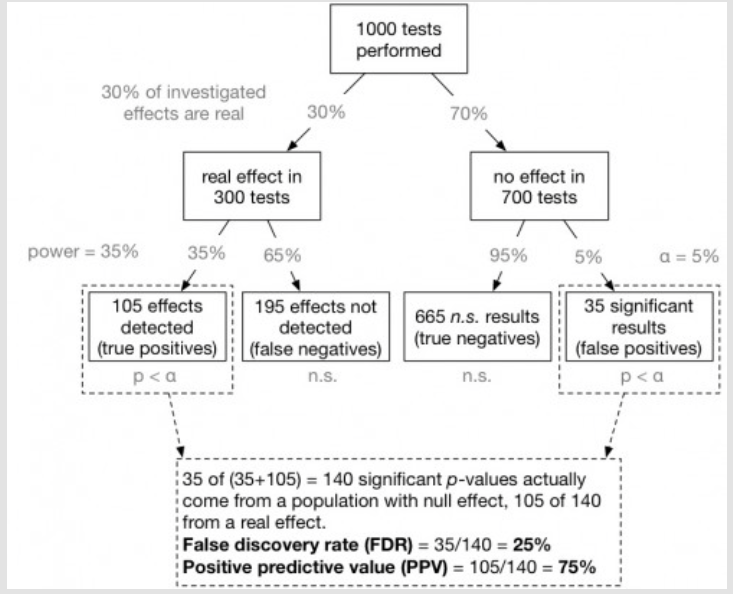
\includegraphics[width=0.5\textwidth]{figures/fig4}
        \caption{False Positives \textit{ Source: http://bit.ly/2ouDzUC}}
    \label{figure 3}
  \end{center}
\end{figure}

Keep in mind...
\begin{itemize}
\item We are trying to calculate $P$(effect $\arrowvert$ significance)
\item $\alpha=P$(significance $\arrowvert$ no effect)
\item Power = $P$(significance $\arrowvert$ effect)\\
\end{itemize}

We can use R to simulate experiments and observe the effects of sample size, power, and significance levels.   Check out the code from this week's lecture for more details, but some of the main ideas discussed were:

\begin{itemize}
\item How does variation change as we change the number of experiments (i.e. the sample size)?   As sample size increases, sampling variation decreases.  However, doubling the sample size does not result in a halving of the width of the distribution.  The standard error as a function of $N$ decreases according to $\frac{1}{\sqrt{N}}$
\item After computing the upper and lower confidence intervals, it is useful to heck how often the true proportion is contained in the confidence interval.  
\item With hypothesis testing, we simulate the null distribution, and then compare this to the real experiment that we do just once.  We then set a threshold, $\alpha$, which is the minimum size the p-value can be to reject the null.
\item In comparing two proportions, we can run experiments for both and then look at the distribution of the outcomes. 
\item Use a \textbf{power proportion test} to compute the $N$ you need to obtain a certain power and significance level.  This will tell us what to set $N$ to in order to detect something $x\%$ of the time (here $x$ is the power level you set). Note, that we see diminishing returns at a point: as we keep increasing $N$, we don't get much more power.  In psychological studies, power is typically in the 30$\%$ range. 
\end{itemize}

A practical tip is to run a \textbf{pilot study} of your experiment.  This is a small version of your experiment, which you can use to get (i) an estimate of the proportions, and (ii) a sense of what you did wrong before you execute experiment at scale.  Then, you can use the power proportion test to see what size $N$ you need.  Make sure you are well-powered, so that you have a lower FDR.  A caveat here is that in some industries, sometimes more thing have a real effect so you don't need power to be as high in order to achieve a low FDR. 

\subsubsection{Researcher degrees of freedom (plus publication bias and p-hacking)}

Researcher degrees of freedom implies that decisions about what statistical tests to compute are made based on the data.  Thus, there is flexibility in the analysis, beyond the flexibility in the sampling data.  In this case, if there was different data, the researcher may have decided to run a different test, and we see this variability.  This is an important point that is often missed, as we do not think about what we would have done in a different scenario with different data.\\

Under this topic, we discussed the UPenn paper titled, \textit{False-Positive Psychology: Undisclosed Flexibility in Data Collection and Analysis Allows Presenting Anything as Significant}.  The objective of this paper was to show that by increasing the flexibility of the researcher, the more and more flukes you observe.  The authors measured lots of different outcomes of their study, and sliced it in different ways to see the likelihood of obtaining a false positive.  This experimental flexibility can be likened to overfitting a regression.

Andrew Gelman published a paper on this topic, titled \textit{The garden of forking paths: Why multiple comparisons can be a problem,
even when there is no “fishing expedition” or “p-hacking” and the research hypothesis was posited ahead of time}.  It is important to maintain a bit of skepticism when you see a random experiment. 

\subsubsection{Limitations of random assignment}

Random assignment has some caveats/limitations:
\begin{itemize}
\item Randomization often isn't feasible/ethical
\item Experiments are costly (time, money)
\item Hard to create convincingly parallel worlds (don't forget the independence assumption)
\item Inevitably people deviate from their random assignments: non-compliers
\end{itemize}

Ron Kohavi's work, \textit{Practical Guide to Controlled Experiments on the Web: Listen to Your Customers not to the HiPPO} includes suggestions for controlling experiments on the web, including running A/A tests, pilot testing and considering day of week effects. 

Next we discussed the paper \textit{Experimental evidence of massive-scale emotional contagion through social networks}, which outlines details of a Facebook experiment.  In this experiment, Facebook manipulated users feed and would either mute or promote words related to various emotions.  Thus, though this manipulated feed, users would see slightly happier or sadder content than the unaltered posts, and then Facebook measured how often users used these emotion-related words.  There was much backlash with this paper as users were uneasy about the manipulation of their feed, and without explicit consent.  While the Facebook terms do legally cover the researchers, there still exist ethical and fairness concerns. 

\section{Natural Experiments}

Sometimes we get lucky and nature or policy effectively runs experiments for us.  The types of natural experiments we discussed were:
as-if random, instrumental variables, discontinuities, and difference in differences.


\subsubsection{As-if random}
\textbf{Idea}: Nature randomly assigns conditions (and people also comply).  

An example of this is the Cholera outbreak in London in 1854, where people were randomly exposed to different water sources, some of which were contaminated. 

\subsubsection{Instrumental variables}
\textbf{Idea}: An instrument independently shifts the distribution of a treatment

For example, if you want to assess the effect of military service on future earnings, intervening with a lottery allows you to measure this effect. The instrumental variable must systematically shift the distribution.  It is important to note that those assigned to treatment is not the same as the treatment people receive (this will be discussed later).

\begin{figure}[ht]
  \begin{center}
    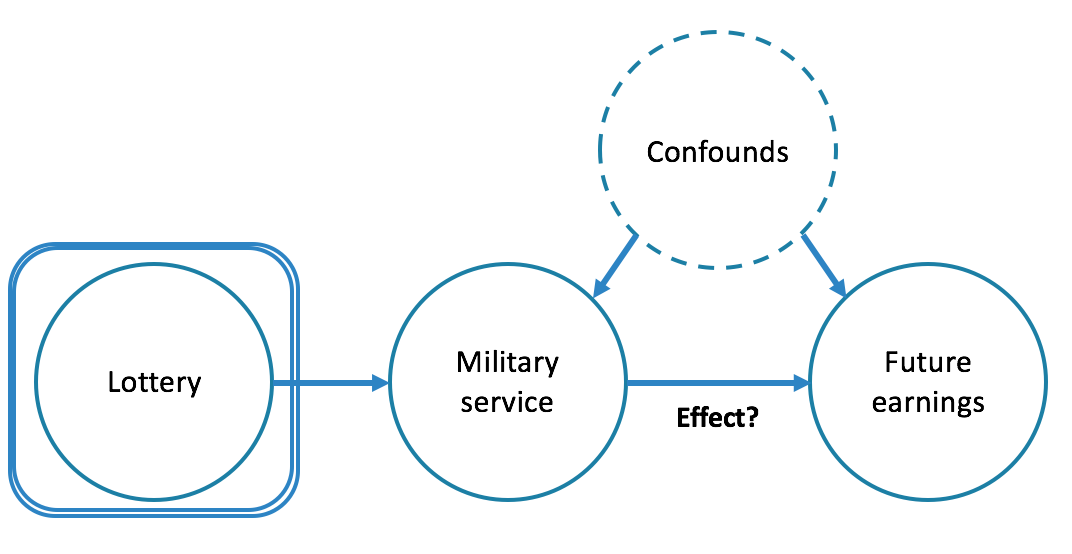
\includegraphics[width=0.5\textwidth]{figures/fig7}
        \caption{Instrumental variables: a lottery influences military service \textit{ Source: lecture 11 slides}}
    \label{figure 7}
  \end{center}
\end{figure}

\subsubsection{Regression discontinuities}
\textbf{Idea}: Things change around an arbitrarily chosen threshold.  

The example we discussed in class is related to Figure 5, where Yelp star ratings were arbitrarily rounded and the result is this jump in revenue.

\begin{figure}[ht]
  \begin{center}
    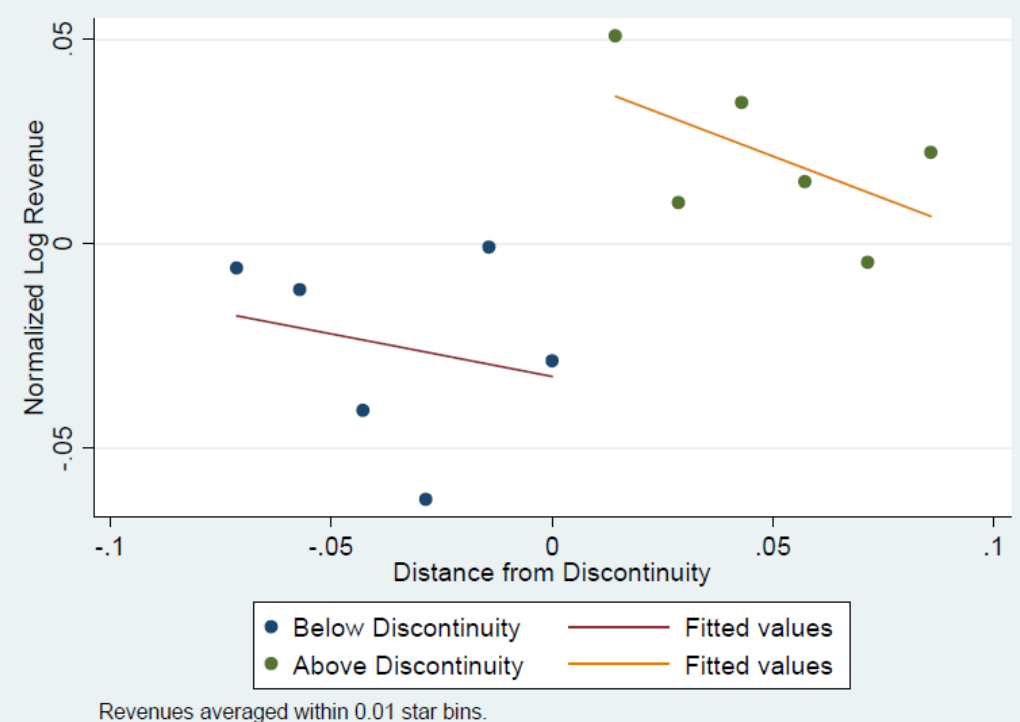
\includegraphics[width=0.5\textwidth]{figures/fig5}
        \caption{Regression discontinuities with Yelp ratings \textit{ Source: http://hbs.me/28NLHND}}
    \label{figure 5}
  \end{center}
\end{figure}

\subsubsection{Difference in differences}
\textbf{Idea}: Compare differences after a sudden change with trends in a control group. 

If wages change in just one state, for example, Figure 6 depicts this shifted trend line where we can see the effect of the treatment.  It is important to note that this change must be sudden, and any anticipation will hurt the validity of the natural experiment results.  This idea is similar to regression discontinuity, but differs in that with difference in differences there was already a trend before. 

\begin{figure}[ht]
  \begin{center}
    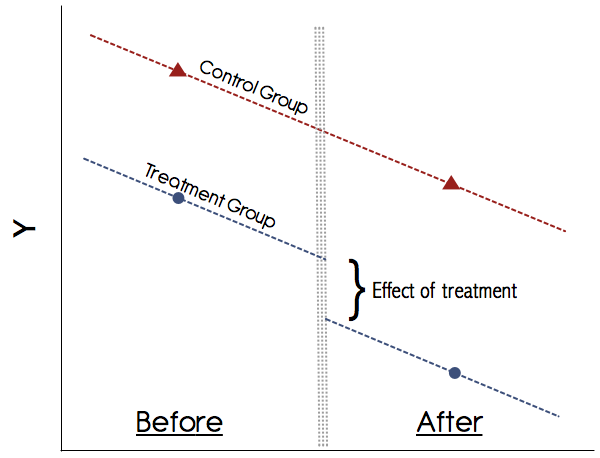
\includegraphics[width=0.5\textwidth]{figures/fig6}
        \caption{Difference in differences trend \textit{ Source: http://bit.ly/2p3YI9o}}
    \label{figure 6}
  \end{center}
\end{figure}

\subsection{Instrumental Variables: In-depth}

\subsubsection{Calculating average treatment effect}

As briefly noted above, assignment to treatment does not equal receipt of treatment. It is important to piece out noncompliance, and the ticket model described in the random assignment section can be used to do this.  Consider three types of people: compliers (c), always-treats (a), and never-treats (n).  We ignore defiers in this world, and assume that people do not do the opposite of what they are told.  Like before, compliers have both tickets: $T_i$ and $C_i$.  Always-treats on the other hand have two $T_i$ tickets, and Never-treats have two $C_i$ tickets.  

In assessing the average treatment effect (ATE), we observe that for always-treats and never-treats, it is zero. Now, to calculate the ATE for compliers, we just use simple algebra:\\

$ATE_{total} = P_c ATE_c + P_a ATE_a + P_n ATE_n$\\

$ATE_{total} = P_c ATE_c + 0 + 0$\\

$ATE_c = \frac{ATE_{total}}{P_c}$\\

Now, in order to calculate the compliance rate, $P_c$ we look at the fraction of those that accept treatment in a group ($P_c+P_a$) less those that accept treatment in the control group ($P_a$).  As a reminder, in the treatment group, those with $T_i$ tickets = $P_c+P_a$, and in the control group, those with $T_i$ tickets = $P_a$. 

\subsubsection{Example: Exercise contagion in a global social network}

As an example of a natural experiment with an instrumental variable, we discussed Christos Nicolaides and Sinan Aral's paper \textit{Exercise contagion in a global social network}.  The idea behind this experiment was to see if social networks have an effect on exercise, using weather patterns as an instrument.  For example, the weather in city A instrumentally shifts the probability of running in city A (i.e. if it is raining, less likely to run). The researchers then measured the effect of their friends in city B running.  In order for this to be valid, it is important to argue that the weather in city B is not a confound for the weather in city A.  Overall, this experiment changes on if your peers run or not, using the weather as an instrument. 

\subsubsection{Caveats}

In practice, it is hard to find instruments.  The instrument cannot have a direct influence on the "effect" action, like future earnings in the military example or running in city B in the exercise contagion example.  Moreover, instrumental variables rely on many untestable assumptions, and you must be certain that no confounds influence the instrument.  Lastly, with natural instrumental variables, the treated population may not be the one you are interested in investigating.

\section{Discovering Natural Experiments}

We can use additional data and algorithms to discover natural experiments.  For example, online retailers are likely interested in learning how much traffic a recommender causes: was a recommender clickthrough causal, or a convenience click.  

To set up this experiment as we have before, we are interested in seeing if a direct view for a focal product has an effect on a referred-click through.  Both are confounded by demand for the products, but an external shock in traffic to the focal product can act as an instrument variable.  By considering this sudden influx of users as an instrument, we are able to measure the marginal effect.  Therefore, we are automatically discovering a natural experiment: first consider a big spike in traffic, then look for a small spike in recommender traffic (this represents an influx of traffic looking at the recommended item) and see if this spike also exists in direct traffic.  

We are able to use data to find these shocks, without knowing what caused it.  In the end, the casual clickthrough is marginal: to calculate the causal effect we look at the change in recommender clicks over the size of the shock

\section{Concluding Remarks}

Large scale observational data is useful for building predictive models, but without random variable it is hard to find causal effects.  We've seen that random experiments are like custom data sets that we can use to answer specific questions. Further, data and algorithms have help us discover and analyze these examples in the wild.

